\section{PyLith Parameter Viewer}
\label{sec:pylith:parameter:viewer}
\newfeature{v2.2.0}

The PyLith Parameter Viewer provides a graphical user interface for
viewing the parameters associated with a PyLith simulation and the
version information for PyLith and its dependencies. This viewer is
an updated and interactive interface to the information generated
by the \filename{pylithinfo} script. It displays the hiearchy of components
and the parameters for each one, including default values.


\section{Installation}

The PyLith Parameter Viewer is included in the PyLith binary
distributions and PyLith Docker container for versions 2.1.5 and
later. Additionally, the PyLith Installer will install the Parameter
Viewer by default.  For manual installation you can download the
PyLith Parameter Viewer tarball from the PyLith software page
(\url{https://geodynamics.org/cig/software/pylith/}).  After
downloading the tarball, unpack it. We recommend unpacking the tarball
in the top-level PyLith directory.
\begin{shell}
$$ tar -xvf pylith_parameters-1.0.0.tgz
\end{shell}

\section{Running the Parameter Viewer}

The steps to run the parameter viewer are:
\begin{enumerate}
\item Generate the parameter JSON file.
\item Start the web server (if not already running).
\item Load the parameter JSON file.
\end{enumerate}

\subsection{Generate the parameter JSON file}

The parameter viewer uses a JSON file with all of the parameters
collected from \filename{.cfg} files, command line arguments, etc as
input. This file can be generated using \filename{pylithinfo} (see
Section \ref{sec:pylithinfo}) and, by default, it will be generated
whenever a \filename{pylith} simulation is run. When using
\filename{pylithinfo}, the name of the parameter file can be set via a
command line argument. When using \filename{pylith}, the
DumpParametersJSON component contains a property for the name of the
file. You can set the filename on the command line
\begin{shell}
$$ pylith --dump_parameters.filename=FILENAME.json
\end{shell}
or within a .cfg file
\begin{cfg}
<h>[pylithapp.dump_parameters]</h>
<p>filename</p> = FILENAME.json
\end{cfg}
Currently, the JSON parameter file cannot be used to run a PyLith
simulation. This feature will be added in an upcoming release.


\subsection{Start the web server}

Change to the directory containing the \filename{pylith\_paramviewer}
script (usually the \filename{parametersgui} directory under the top-level
\filename{pylith} directory), and run the \filename{pylith\_paramviewer}
script. This will start a simple Python-based web server on your local
computer.
\begin{shell}
$$ cd parametersgui
$$ ./pylith\_paramviewer
\end{shell}
The script will instruct you to point your web browswer to a local
port on your computer. The default is \url{http://127.0.0.1:9000}.
You can change the default port using the \filename{-{}-port} command
line argument to the \filename{pylith\_paramviewer} script.


\section{Using the Parameter Viewer}

When you point your web browser to the correct port, you should see
the PyLith Parameter Viewer as shown in Figure
\ref{fig:parameters:gui:startup}.  Click the \textsf{Choose File}
button and navigate to the desired JSON parameter file. The viewer
tarball includes a sample parameter file
\filename{sample\_parameters.json}. Click the \textsf{Reload} button
to reload the same JSON parameter file if you regenerate it. To select
a new JSON parameter file, click the \textsf{Choose File} button and
navigate to the desired file.

\begin{figure}[htbp]
  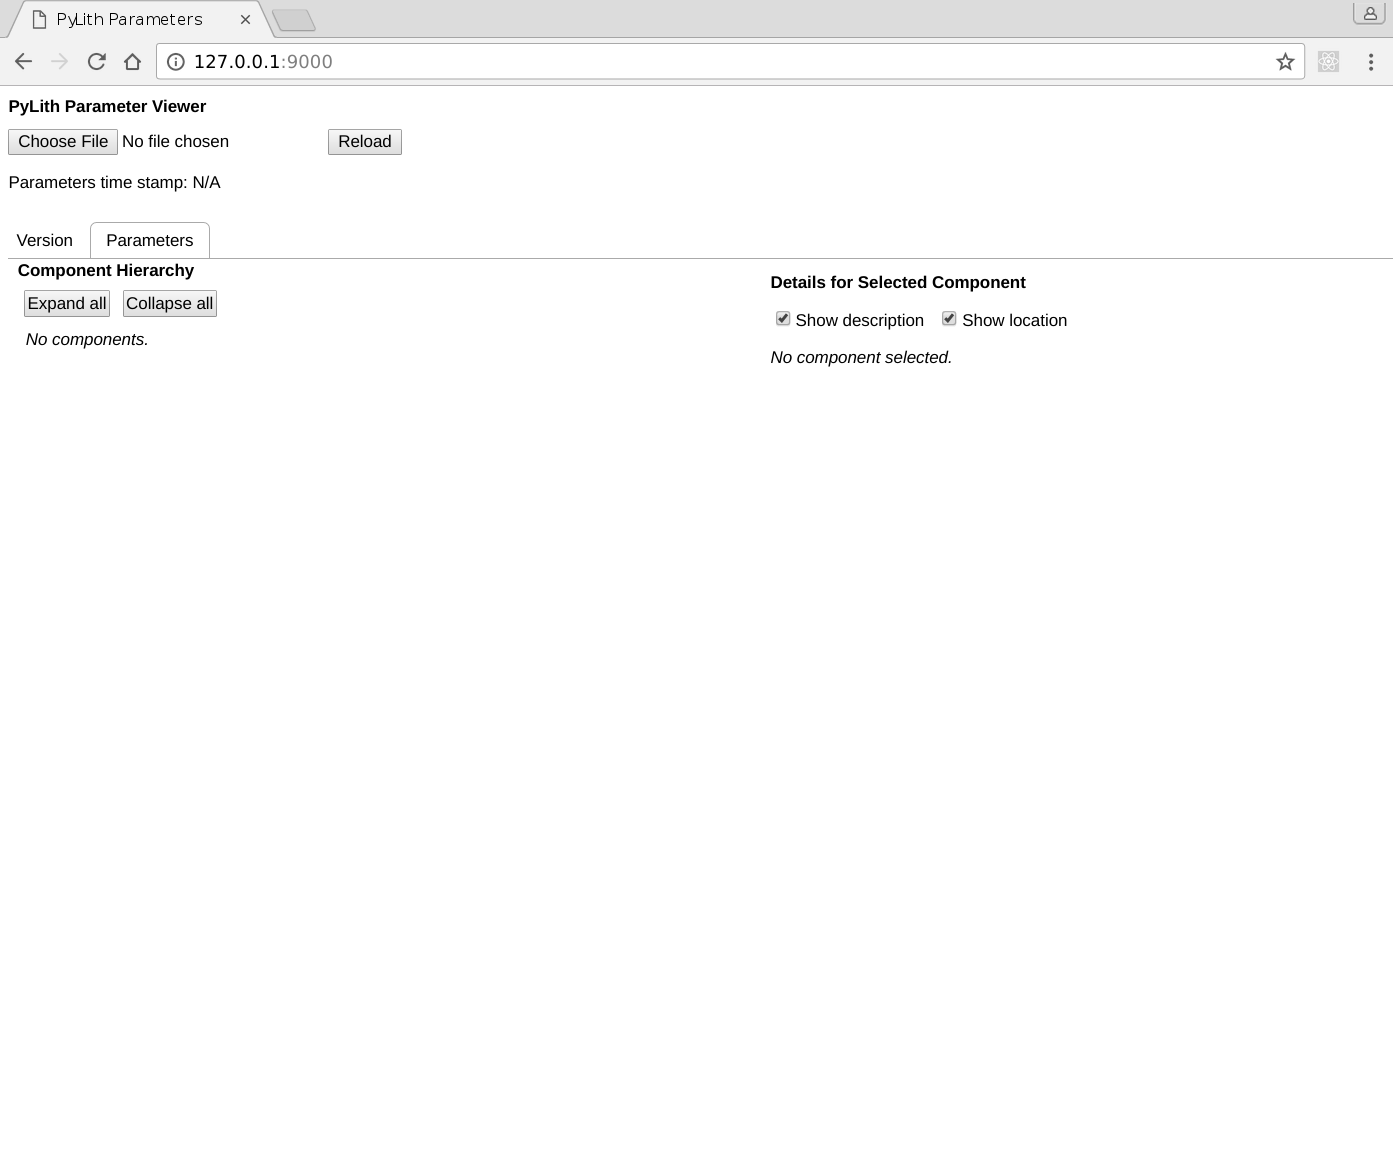
\includegraphics[width=5in]{runpylith/figs/paramgui_startup} 
  \caption{Screenshot of PyLith Parameter Viewer in web browser upon startup.}
  \label{fig:parameters:gui:startup} 
\end{figure}


\subsection{Version Information}

Click on the \textsf{Version} tab to examine the version information.
This tab displays the same version information shown with the
\filename{-{}-version} command line argument to \filename{pylith} in
an easy to read layout.  This includes information about the platform
on which \filename{pylith} or \filename{pylithinfo} was run, the
PyLith version, and versions of the dependencies, as shown in Figure
\ref{fig:parameters:gui:version}.

\begin{figure}[htbp]
  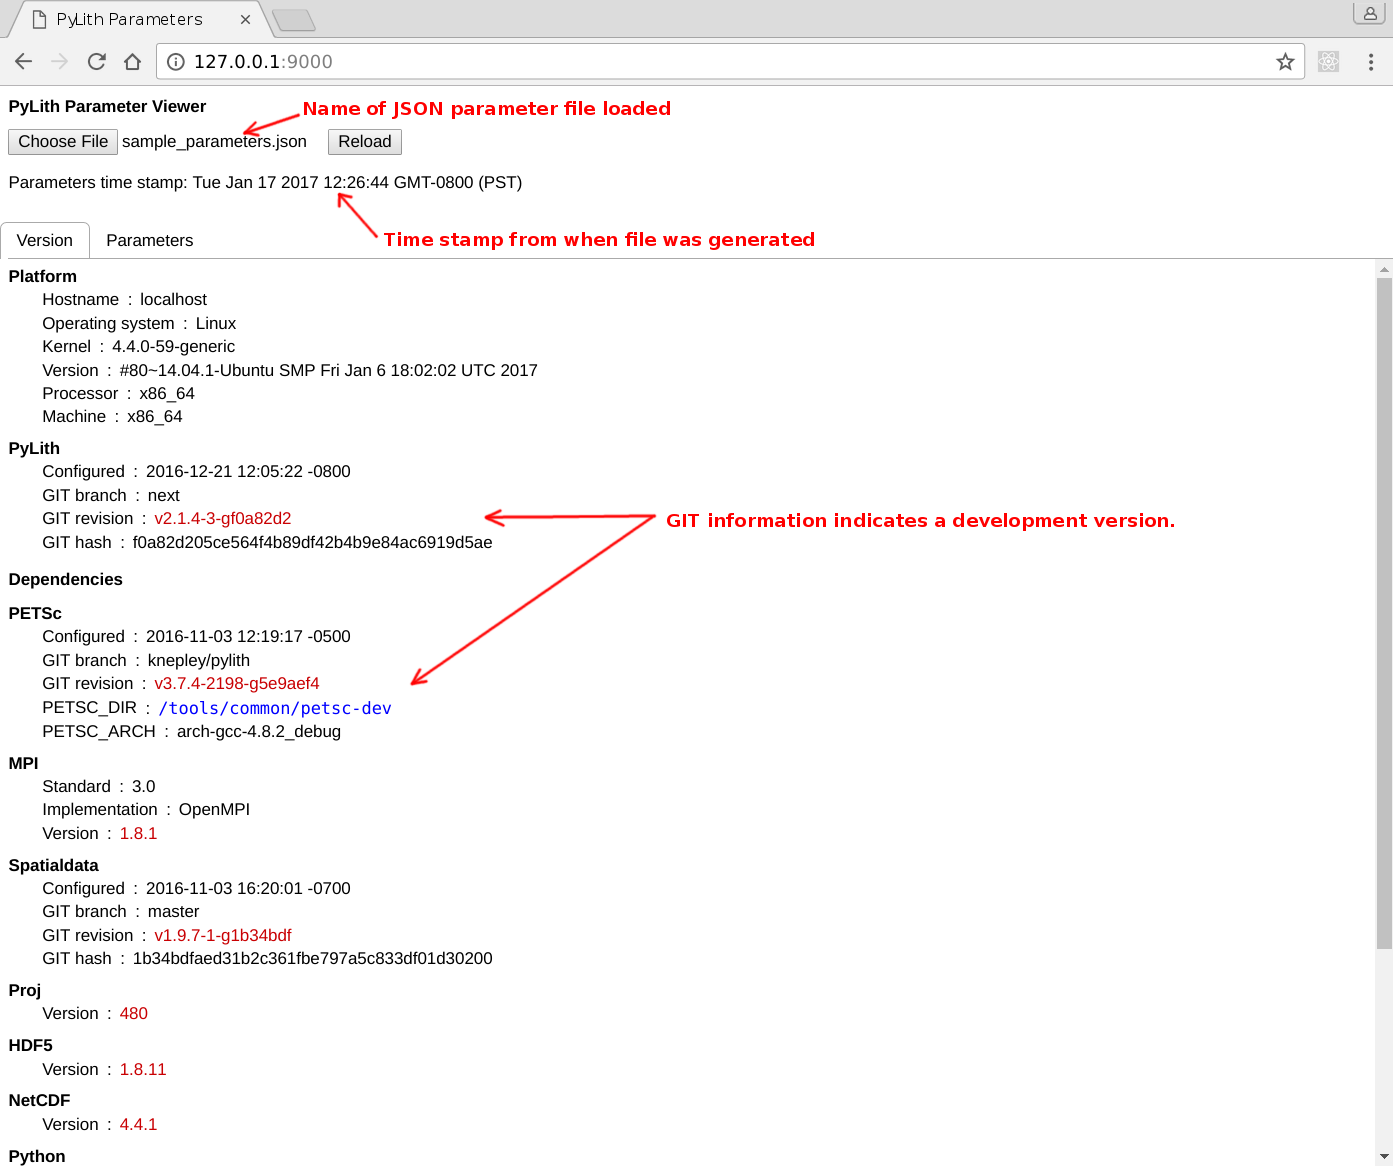
\includegraphics[width=5in]{runpylith/figs/paramgui_version} 
  \caption{Screenshot of \textsf{Version} tab of the PyLith Parameter Viewer
    with sample JSON parameter file.}
  \label{fig:parameters:gui:version} 
\end{figure}


\subsection{Parameter Information}

Click on the \textsf{Parameters} tab to examine the hiearchy of
components and the parameters for each. You can expand/collapse the
Component Hierarchy tree in the left panel by clicking on the
triangles or facility name in blue to the left of the equals sign
(Figure \ref{fig:parameters:gui:parameters:empty}).  Clicking on the
component in red to the right of the equals sign will show its
parameters in the right panel (Figure
\ref{fig:parameters:gui:parameters:empty}).  The selected facility in
the left panel whose parameters are shown in the right panel will be
highlighted via a gray background (Figure
\ref{fig:parameters:gui:parameters:selected}).

\begin{figure}[htbp]
  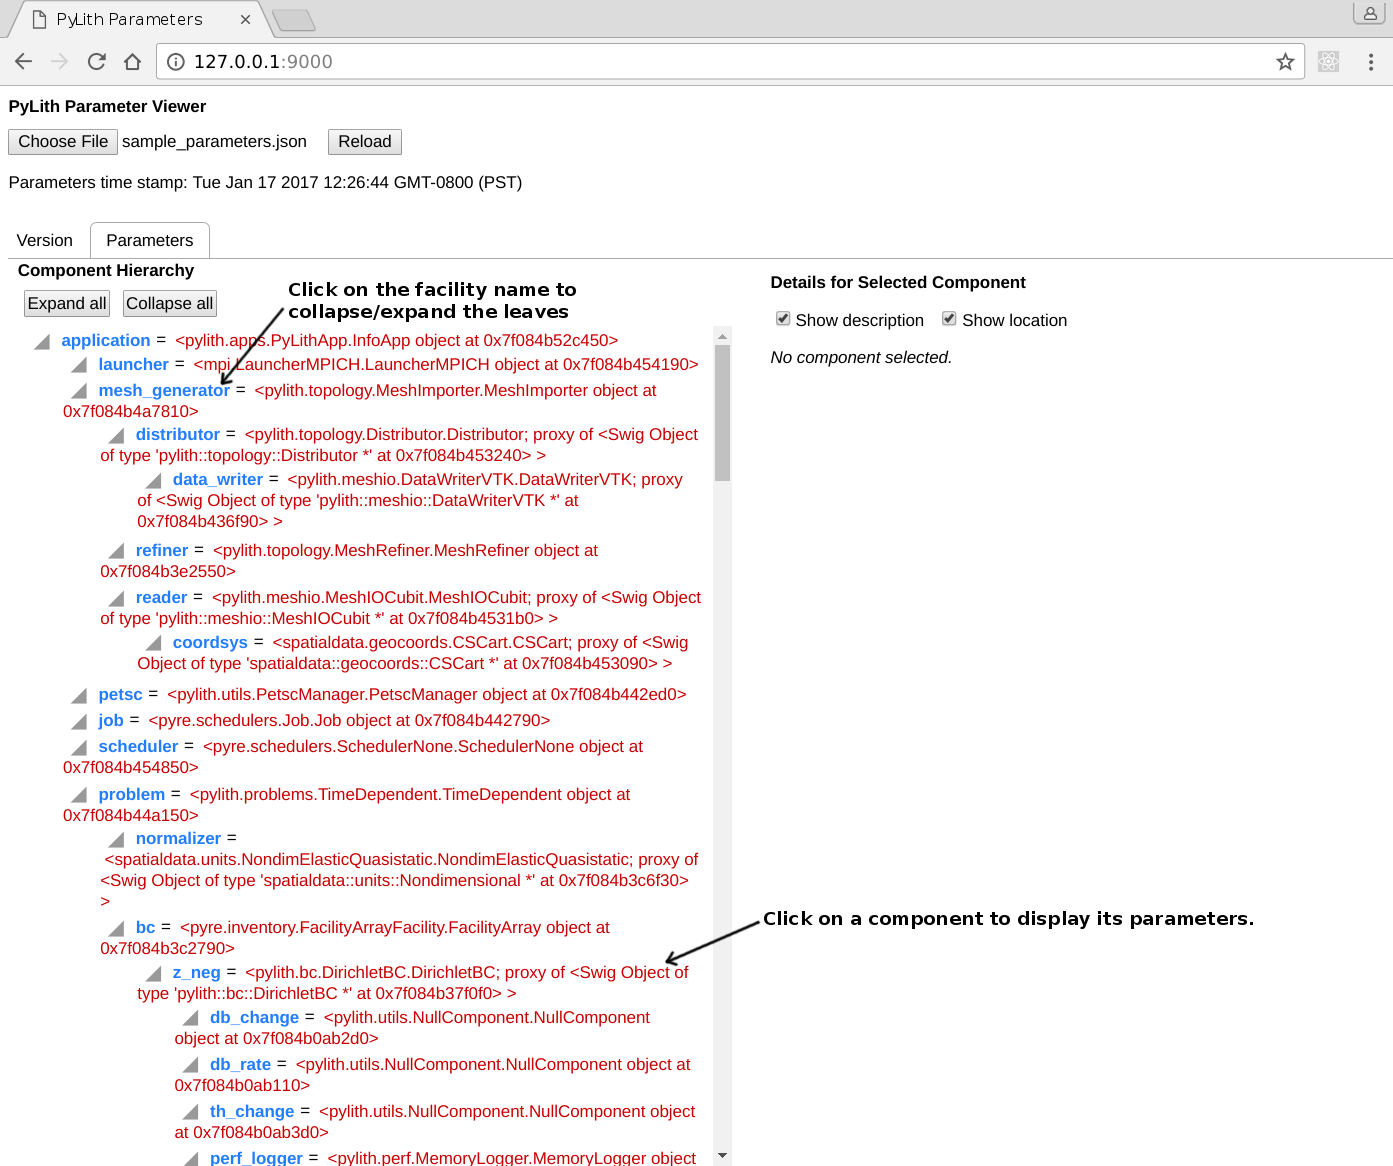
\includegraphics[width=5in]{runpylith/figs/paramgui_parameters} 
  \caption{Screenshot of \textsf{Parameters} tab of the PyLith Parameter Viewer
    with sample JSON parameter file before selecting a component in the
    left panel.}
  \label{fig:parameters:gui:parameters:empty}
\end{figure}


\begin{figure}[htbp]
  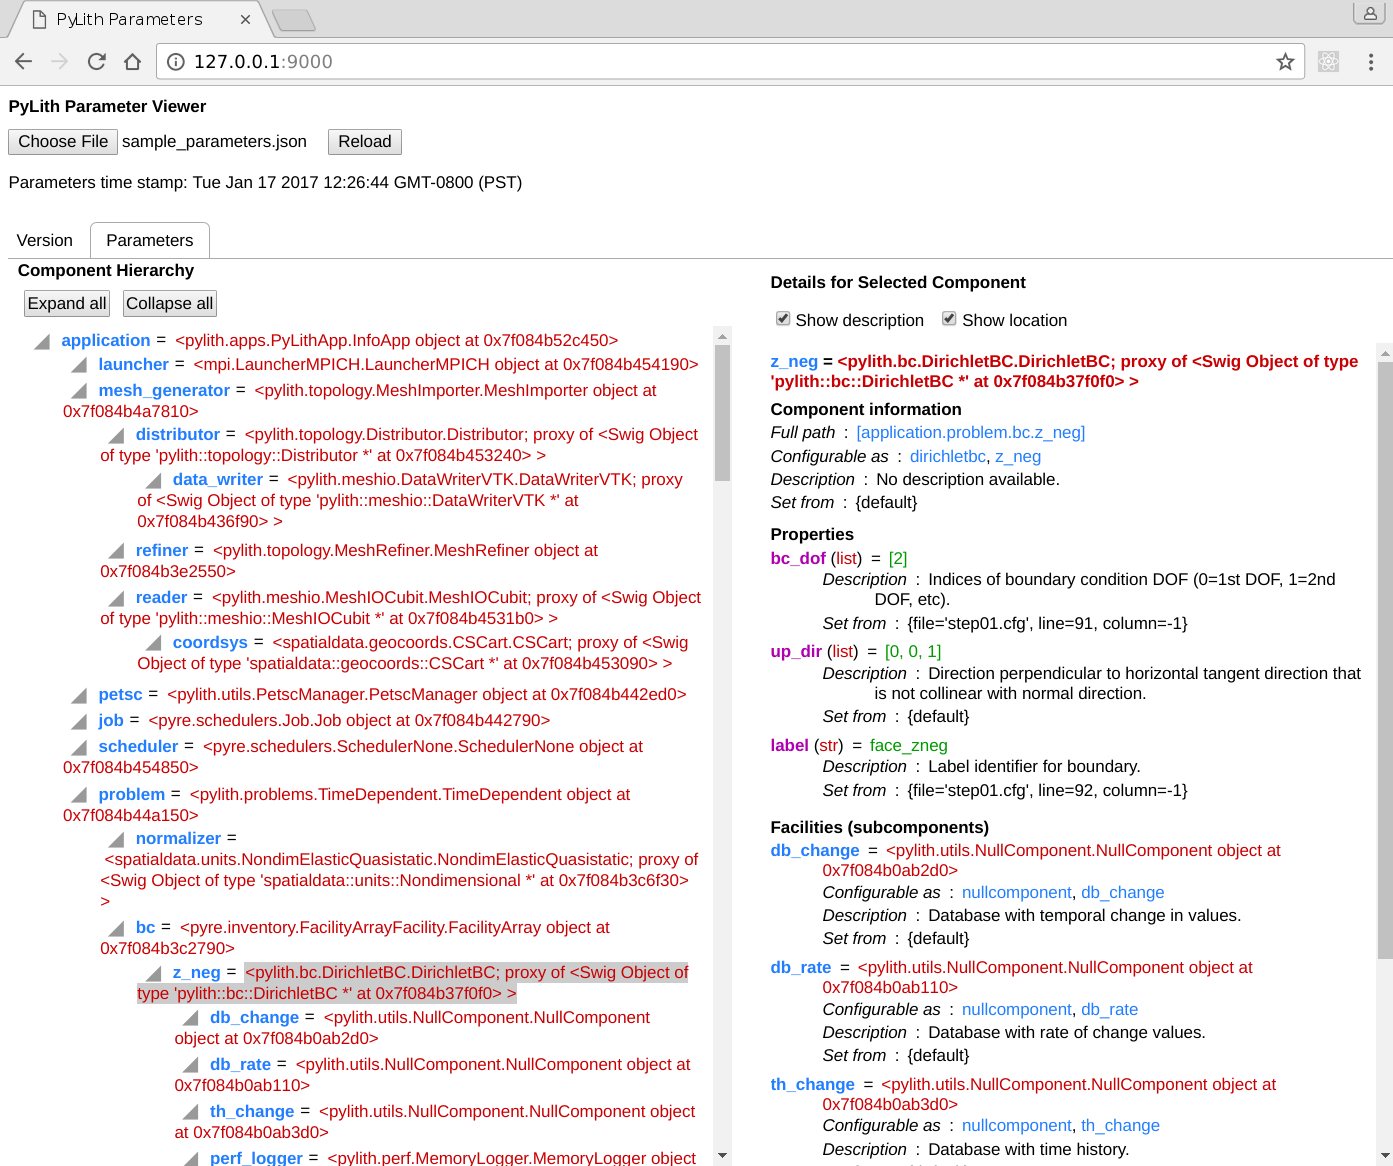
\includegraphics[width=5in]{runpylith/figs/paramgui_detail} 
  \caption{Screenshot of \textsf{Parameters} tab of the PyLith Parameter Viewer
    with sample JSON parameter file with the \facility{z\_neg} facility
    selected.}
  \label{fig:parameters:gui:parameters:selected} 
\end{figure}


% End of file